
\documentclass[12pt, a4paper]{report}
\usepackage{epsfig}
\usepackage{subfigure}
%\usepackage{amscd}
\usepackage{amssymb}
\usepackage{graphicx}
%\usepackage{amscd}
\usepackage{amssymb}
\usepackage{subfiles}
\usepackage{framed}
\usepackage{subfiles}
\usepackage{amsthm, amsmath}
\usepackage{amsbsy}
\usepackage{framed}
\usepackage[usenames]{color}
\usepackage{listings}
\lstset{% general command to set parameter(s)
basicstyle=\small, % print whole listing small
keywordstyle=\color{red}\itshape,
% underlined bold black keywords
commentstyle=\color{blue}, % white comments
stringstyle=\ttfamily, % typewriter type for strings
showstringspaces=false,
numbers=left, numberstyle=\tiny, stepnumber=1, numbersep=5pt, %
frame=shadowbox,
rulesepcolor=\color{black},
,columns=fullflexible
} %
%\usepackage[dvips]{graphicx}
\usepackage{natbib}
\bibliographystyle{chicago}
\usepackage{vmargin}
% left top textwidth textheight headheight
% headsep footheight footskip
\setmargins{3.0cm}{2.5cm}{15.5 cm}{22cm}{0.5cm}{0cm}{1cm}{1cm}
\renewcommand{\baselinestretch}{1.5}
\pagenumbering{arabic}
\theoremstyle{plain}
\newtheorem{theorem}{Theorem}[section]
\newtheorem{corollary}[theorem]{Corollary}
\newtheorem{ill}[theorem]{Example}
\newtheorem{lemma}[theorem]{Lemma}
\newtheorem{proposition}[theorem]{Proposition}
\newtheorem{conjecture}[theorem]{Conjecture}
\newtheorem{axiom}{Axiom}
\theoremstyle{definition}
\newtheorem{definition}{Definition}[section]
\newtheorem{notation}{Notation}
\theoremstyle{remark}
\newtheorem{remark}{Remark}[section]
\newtheorem{example}{Example}[section]
\renewcommand{\thenotation}{}
\renewcommand{\thetable}{\thesection.\arabic{table}}
\renewcommand{\thefigure}{\thesection.\arabic{figure}}
\title{Research notes: linear mixed effects models}
\author{ } \date{ }


\begin{document}
\author{Kevin O'Brien}
\title{Mixed Models for Method Comparison Studies}
\tableofcontents

%----------------------------------------------------------------------------------------%
\newpage

\chapter{Model Diagnostics}
%---------------------------------------------------------------------------%
%1.1 Introduction to Influence Analysis
%1.2 Extension of techniques to LME Models
%1.3 Residual Diagnostics
%1.4 Standardized and studentized residuals
%1.5 Covariance Parameters
%1.6 Case Deletion Diagnostics
%1.7 Influence Analysis
%1.8 Terminology for Case Deletion
%1.9 Cook's Distance (Classical Case)
%1.10 Cook's Distance (LME Case)
%1.11 Likelihood Distance
%1.12 Other Measures
%1.13 CPJ Paper
%1.14 Matrix Notation of Case Deletion
%1.15 CPJ's Three Propositions
%1.16 Other measures of Influence
%---------------------------------------------------------------------------%

\section{Model Validation}
%http://www.itl.nist.gov/div898/handbook/pmd/section4/pmd44.htm
Model validation is possibly the most important step in the model building sequence. It is also one of the most overlooked. Often the validation of a model seems to consist of nothing more than quoting the $R^2$ statistic from the fit (which measures the fraction of the total variability in the response that is accounted for by the model). Unfortunately, a high $R^2$ value does not guarantee that the model fits the data well. Use of a model that does not fit the data well will not provide any meaningful insights to the underlying research questions.


In classical linear models, model diagnostics techniques determine whether or not the distributional assumptions are satisfied, and to assess the influence of unusual observations, and have been become a required part of any statistical analysis. Well established methods are commonly available in statistical packages and standard textbooks on applied regression. However it has been noted by several papers that model diagnostics do not often accompany LME model analyses. \citet{schabenberger} discusses the state of LME diagnostics tools, providing a useful summary of established measures.

%\subsection{Model Data Agreement} %1.1.1
\citet{schabenberger} describes the examination of model-data agreement as comprising several elements; residual analysis, goodness of fit, collinearity diagnostics and influence analysis.





%% \subsection{Why Use Residuals?}
%If the model fit to the data were correct, the residuals would approximate the random errors that make the relationship between the explanatory variables and the response variable a statistical relationship. Therefore, if the residuals appear to behave randomly, it suggests that the model fits the data well. On the other hand, if non-random structure is evident in the residuals, it is a clear sign that the model fits the data poorly. The subsections listed below detail the types of plots to use to test different aspects of a model and give guidance on the correct interpretations of different results that could be observed for each type of plot.
%------------------------------------------------------------------------------------------------------------------------ %


	\section{Residual diagnostics} %1.3

	%A residual is the difference between an observed quantity and its estimated or predicted value. 
	%A residual is simply the difference between an observed value and the corresponding fitted value, as predicted by the model.
	Residual analysis is a widely used model validation technique. For classical linear models, residual diagnostics are typically implemented as a plot of the observed residuals and the predicted values. A visual inspection for the presence of trends inform the analyst on the validity of distributional assumptions, and to detect outliers and influential observations. The rationale is that, if the model is properly fitted to the model, then the residuals would approximate the random errors that one should expect; if the residuals behave randomly, with no noticeable patterns or trends. If some sort of non-random trend is evident in the model, then the model can be considered to be poorly fitted. 	For classical linear models, residual diagnostics are typically implemented as a plot of the observed residuals and the predicted values. A visual inspection for the presence of trends inform the analyst on the validity of distributional assumptions, and to detect outliers and influential observations. Statistical software environments, such as the \texttt{R} programming language, provides a suite of tests and graphical procedures for appraising a fitted linear model, with several of these procedures analysing the model residuals. 	However, for LME models the matter of residual is more complex, both from a theoretical point of view and from the practical matter of implementing a comprehensive analysis using statistical software. As the LME model can be tailored to the needs of the particular research question, the rationale behind the model appraisal must follow accordingly.
	
	
	For an LME model, the \textit{raw} residuals at level $i$ are obtained by subtracting the fitted levels at that level from the response vector If we require a \textit{Pearson} type residual, we further dviide this by the estimated within-group standard error. The Pearson residual is the raw residual divided by the square root of the the within-group standard error for both methods. The fitted values at level $i$ are obtained by adding together the population fitted values (based only on the fixed effects estimates) and the estimated contributions of the random effects to the fitted values at grouping levels less or equal to $i$. In addition to Raw and Pearson residuals, there are normalized residuals : standardized residuals pre-multiplied by the inverse square-root factor of the estimated error correlation matrix. For the forthcoming examples, we will use the raw residuals.
	
	
	%-----------------------------------------------------------------------------------------%
	
	\section*{Preliminary Residual Analysis }
	
	% This short section will look at residual analysis for LME models. 
	The underlying assumptions for LME models are similar to those of classical linear mdoels. There are two key techniques: a residual plot and the normal probability plot. Using the nlme package it is possible to create plots specific to each method. This is useful in determine which methods `disagree` with the rest.
	Analysis of the residuals would determine if the methods of measurement disagree systematically, or whether or not erroneous measurements associated with a subset of the cases are the cause of disagreement.
	Erroneous measurements are incorrect measurements that indicate disagreement between methods that would otherwise be in agreement.
	%======================================================== %
	Once the residuals are computed, they can be used to make an assessment about the model fit. For the LME model described in Chapter 2, we can plot the residuals against the fitted values, to assess the assumption of constant variance. f the points in a residual plot are randomly dispersed around the horizontal axis, a linear regression model is appropriate for the data; otherwise, a non-linear model is more appropriate.
	
	\begin{figure}[h!]
		\centering
		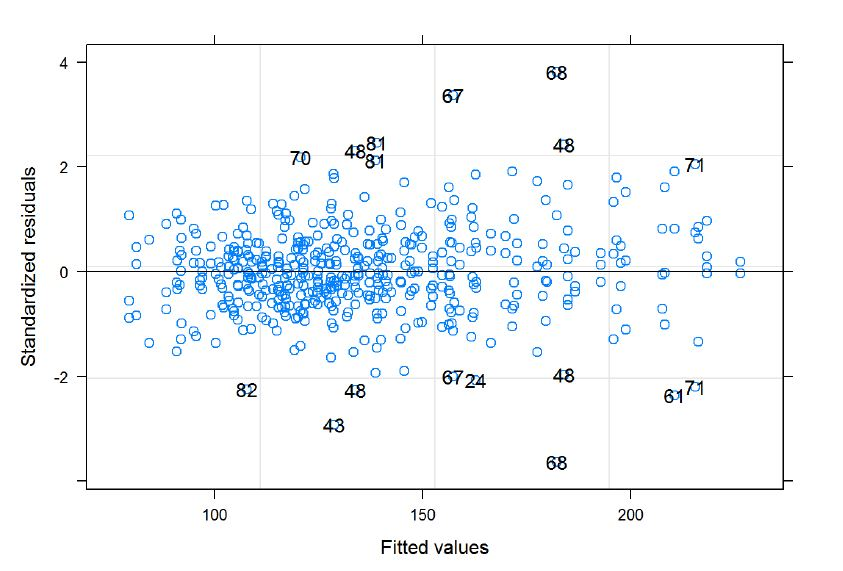
\includegraphics[width=0.9\linewidth]{images/Residuals-JS-Roy}
		\caption{}
		\label{fig:Residuals-JS-Roy}
	\end{figure}
	
	LME models assume that the residuals of the model are normally distributed.  The residuals can be divided according to groups according to the method of measurement. In the following examples, we seperately assess normality the \textit{J} method residuals (the first 255 residuals) and \textit{S} method residuals (the remaining 255). Importantly the residuals from the \textit{J} method are normally distributed, but there is non-normality of the residuals according to the \textit{S} method.
	\begin{framed}
		\begin{verbatim}
		> shapiro.test(resid(JS.roy1)[1:255])
		
		Shapiro-Wilk normality test
		
		data:  resid(JS.roy1)[1:255]
		W = 0.9931, p-value = 0.2852
		\end{verbatim}
	\end{framed}
	
	\begin{framed}
		\begin{verbatim}
		> shapiro.test(resid(JS.roy1)[256:510])
		
		Shapiro-Wilk normality test
		
		data:  resid(JS.roy1)[256:510]
		W = 0.9395, p-value = 9.503e-09
		\end{verbatim}
	\end{framed}
	\begin{figure}[h!]
		\centering
		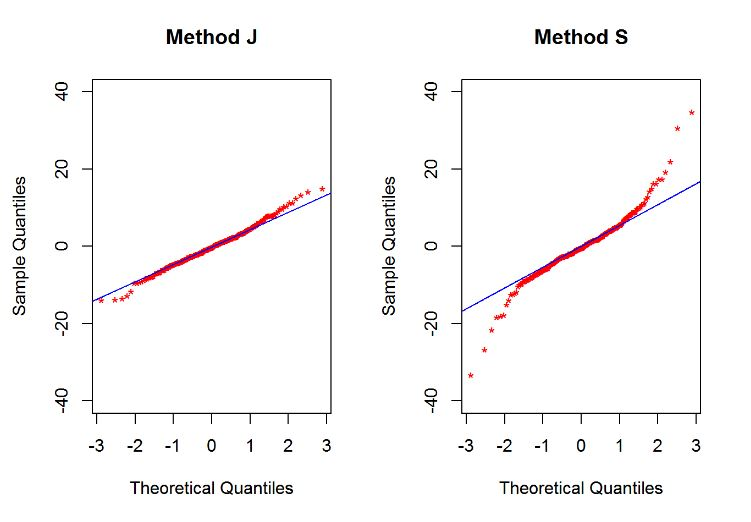
\includegraphics[width=0.9\linewidth]{images/Resid-newplot2}
		
	\end{figure}
	
	%===================================================================================================%
	
	
	
	\begin{figure}[h!]
		\centering
		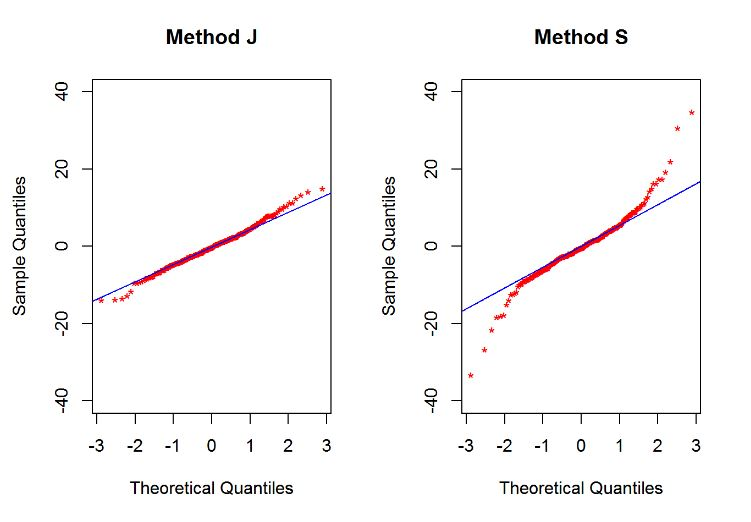
\includegraphics[width=1.1\linewidth]{images/Resid-newplot2}
		\caption{}
		\label{fig:Resid-newplot2}
	\end{figure}
	
	\begin{figure}[h!]
		\centering
		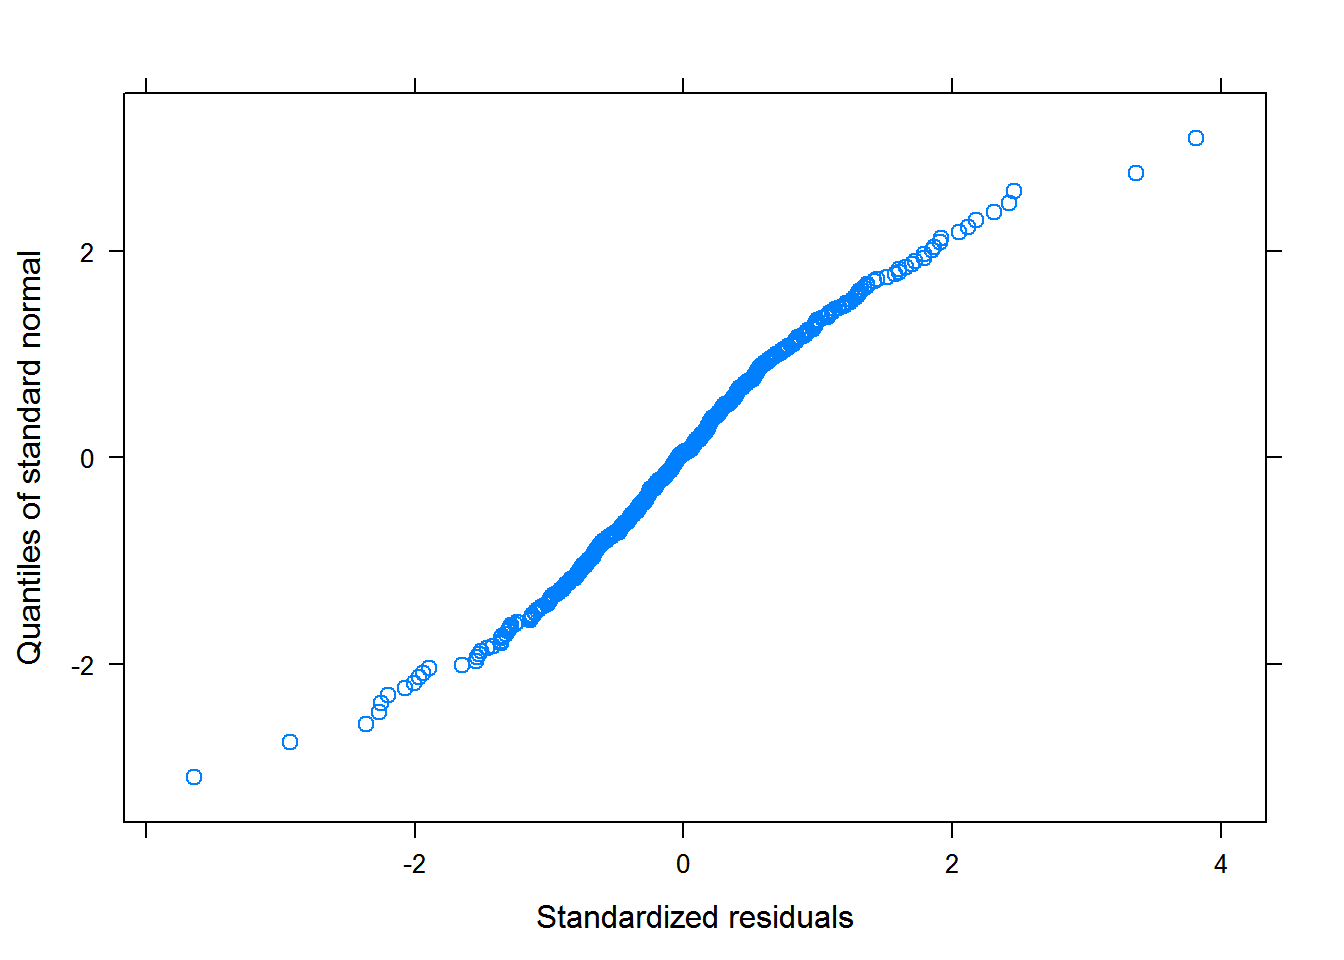
\includegraphics[width=0.9\linewidth]{images/ResidPlot3}
		\label{fig:ResidPlot3}
	\end{figure}
	
	Normal probability plots can be rendered for each level of the random effects.  LME models assume that not only the within-cluster residuals are normally distributed, but that each level of the random effects are as well. % 
	\begin{figure}[h!]
		\centering
		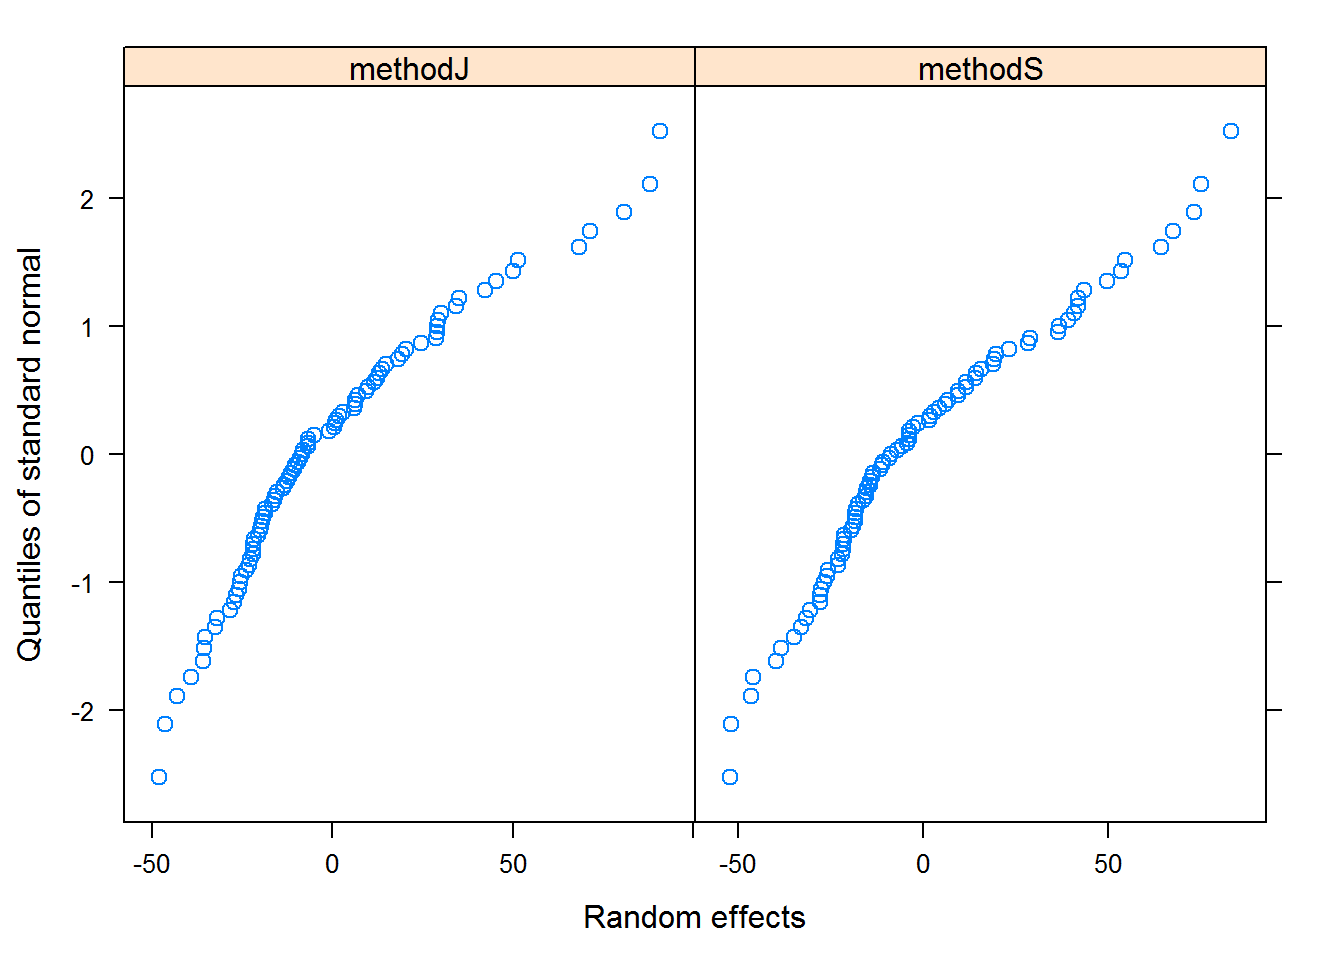
\includegraphics[width=0.9\linewidth]{images/ResidPlot2}
		\caption{}
		\label{fig:ResidPlot2}
	\end{figure}




%
%\subsection{Introduction}
%In statistics and optimization, statistical errors and residuals are two closely related and easily confused measures of the deviation of an observed value of an element of a statistical sample from its "theoretical value". The error (or disturbance) of an observed value is the deviation of the observed value from the (unobservable) true function value, while the residual of an observed value is the difference between the observed value and the estimated function value.
%
%The distinction is most important in regression analysis, where it leads to the concept of studentized residuals.
%
%









%---------------------------------------------------------------------------%







\section{Standardization and Studentization} %1.4.2
To alleviate the problem caused by inconstant variance, the residuals can be scaled (i.e. divided) by their standard deviations. This results in a \index{standardized residual}`standardized residual'. A random variable is said to be standardized if the difference from its mean is scaled by its standard deviation. The residuals  have mean zero but their variance is unknown, it depends on the true values of $\theta$. Standardization is  not possible in practice. Because true standard deviations are frequently unknown, one can instead divide a residual by the estimated standard deviation to obtain the \index{studentized residual}`studentized residual. 
%Instead, you can compute studentized residuals by dividing a residual by an estimate of its standard deviation. 
If that estimate is independent of the $i-$th observation, the process is termed \index{external studentization}`external studentization'. This is usually accomplished by excluding the $i-$th observation when computing the estimate of its standard error. If the observation contributes to the
standard error computation, the residual is said to be \index{internally studentization}internally studentized.
Externally \index{studentized residual} studentized residual require iterative influence analysis or a profiled residuals variance \textbf{(CITE)}.


% \subsection{Computation}%1.4.4

The computation of internally studentized residuals relies on the diagonal entries of $\boldsymbol{V} (\hat{\theta})$ - $\boldsymbol{Q} (\hat{\theta})$, where $\boldsymbol{Q} (\hat{\theta})$ is computed as

\[ \boldsymbol{Q} (\hat{\theta}) = \boldsymbol{X} ( \boldsymbol{X}^{\prime}\boldsymbol{Q} (\hat{\theta})^{-1}\boldsymbol{X})\boldsymbol{X}^{-1} \]


\subsection{Pearson Residual}%1.4.5

Another possible scaled residual is the \index{Pearson residual} `Pearson residual', whereby a residual is divided by the standard deviation of the dependent variable. The Pearson residual can be used when the variability of $\hat{\beta}$ is disregarded in the underlying assumptions.



	

	%-----------------------------------------------------------------------------------------%
In this chapter, we will look at residual analysis and diagnostic toold for LME models, and discuss how they can be applied to the Method Comparison Problem.	In classical linear models, a residual is the difference between an observed value and its estimated or predicted value. For LME models, the topic is more complicated, and still a matter of active research. 


	\section{Distinction From Linear Models (Schabenberger page 3)}
	%% Where is this coming from?
	%% 
 The differences between perturbation and residual analysis in the linear model and the linear mixed model
		are connected to the important facts that b and b
		depend on the estimates of the covariance parameters,
		that b has the form of an (estimated) generalized least squares (GLS) estimator, and that 
		is a random
		vector.
 In a mixed model, you can consider the data in a conditional and an unconditional sense. If you imagine
		a particular realization of the random effects, then you are considering the conditional distribution
		Y|
 If you are interested in quantities averaged over all possible values of the random effects, then
		you are interested in Y; this is called the marginal formulation. In a clinical trial, for example, you
		may be interested in drug efficacy for a particular patient. If random effects vary by patient, that is a
		conditional problem. If you are interested in the drug efficacy in the population of all patients, you are
		using a marginal formulation. Correspondingly, there will be conditional and marginal residuals, for
		example.
The estimates of the fixed effects  depend on the estimates of the covariance parameters. If you are
		interested in determining the influence of an observation on the analysis, you must determine whether
		this is influence on the fixed effects for a given value of the covariance parameters, influence on the
		covariance parameters, or influence on both.
Mixed models are often used to analyze repeated measures and longitudinal data. The natural experimental
		or sampling unit in those studies is the entity that is repeatedly observed, rather than each
		individual repeated observation. For example, you may be analyzing monthly purchase records by
		customer. 
An influential “data point” is then not necessarily a single purchase. You are probably more
		interested in determining the influential customer. This requires that you can measure the influence
		of sets of observations on the analysis, not just influence of individual observations.
%		\item The computation of case deletion diagnostics in the classical model is made simple by the fact that
%		%estimates of  and 2, which exclude the ith observation, can be %computed without re-fitting the
%		model. Such update formulas are available in the mixed model only if you assume that the covariance
%		parameters are not affected by the removal of the observation in question. This is rarely a reasonable
%		assumption.
The application of well-known concepts in model-data diagnostics to the mixed model can produce results
		that are at first counter-intuitive, since our understanding is steeped in the ordinary least squares
		(OLS) framework. As a consequence, we need to revisit these important concepts, ask whether they
		are “portable” to the mixed model, and gain new appreciation for their changed properties. An important
		example is the ostensibly simple concept of leverage. 
%		\item The definition of leverage adopted by
%		the MIXED procedure can, in some instances, produce negative values, which are mathematically
%		impossible in OLS. Other measures that have been proposed may be non-negative, but trade other
%		advantages. Another example are properties of residuals. While OLS residuals necessarily sum to
%		zero in any model (with intercept), this not true of the residuals in many mixed models.

	

	
\section{Taxonomy of LME Residuals}

		
		Standard residual and influence diagnostics for linear models can
		be extended to linear mixed models. The dependence of
		fixed-effects solutions on the covariance parameter estimates has
		important ramifications in perturbation analysis. To gauge the
		full impact of a set of observations on the analysis, covariance
		parameters need to be updated, which requires refitting of the
		model.
		%---http://www.stat.purdue.edu/~bacraig/notes598S/SUGI_Paper_Schabenberger.pdf
		
		The conditional (subject-specific) and marginal
		(population-averaged) formulations in the linear mixed model
		enable you to consider conditional residuals that use the
		estimated BLUPs of the random effects, and marginal residuals
		which are deviations from the overall mean. Residuals using the
		BLUPs are useful to diagnose whether the random effects components
		in the model are specified correctly, marginal residuals are
		useful to diagnose the fixed-effects components.	
		
	\citet{pb} describes three types of residual that describe the variabilities
	present in LME models
	\begin{enumerate}
		\item marginal residuals, $\hat{\xi}$, which predict marginal errors,
		\item conditional residuals, $\hat{\epsilon}$, which predict conditional errors,
		\item the BLUP,$\boldsymbol{Z\hat{b}}$, that predicts random effects.
	\end{enumerate}
	Each type of residual is useful to evaluates some assumption of the model.
	
	%- http://www.ime.usp.br/~jmsinger/MAE5705/EMR2013.pdf
	
	According to Hilton \& Minton (1995), a residual is considered pure for a specfic type fo error
	if it depends only on the fixed components and on the error that it is supposed to predict.
	Residuals that depend on other types of error are known as `confounded errors'.



	\section{Residuals in LME Models : Marginal, Conditional and Scaled}
	%------------------------------------------------------------Section 4.3---%
\subsection{Internally and Externally Studentized Residuals}
%Internally and Externally Studentized Residuals
The computation of internally studentized residuals relies on the diagonal values of $\boldsymbol{V(\hat{\theta})} - \boldsymbol{Q(\hat{\theta})}$
Externally studentized residuals require iterative influece analysis or a profiled residual variance.

Cook's Distance
\[ \boldsymbol{\delta}_{(U)} = \boldsymbol{\hat{\beta}}  - \boldsymbol{\hat{\beta}}_{(U)} \]
A DFFIT measures the change in predicted values due to the removal of data points.
(Belsey, Kuh and Welsch (1980))
%[ \mbox{DFFITS}_{i} = \frac{\hat{y}_i - \hat{y}_{i(U)}}{ese(\hat{y}_i)} \]

$\boldsymbol{D(\beta)}  = \boldsymbol{\delta}^{\prime}_{(U)} \boldsymbol{\delta}_{(U)} / rank(\boldsymbol{X})$
Cook's D can be calibrated according to a chi-square distribution with degress of freedom equal to the rank of $\boldsymbol{X}$ \citet{CPJ}.

%	$ \mbox{CovTrace}(\boldsymbol{\beta})$


	%========================================================================================== %
	\section*{Residuals}
	
 The raw residuals $r_{mi}$ and $r_{ci}$ are usually not well suited for these purposes.
	
	\begin{itemize}
		\item Conditional Residuals $r_{ci}$
		\item Marginal Residuals $r_{mi}$
	\end{itemize}
	
	
	%--Marginal and Conditional Residuals
	
	
	
\chapter{Residuals diagnostics in LME Models}
	Residuals are used to examine model assumptions and to detect outliers and potentially influential data
	point. In LME models, there are two types of residuals, marginal residuals and conditional residuals. A marginal residual is the difference between the observed data and the estimated marginal mean. A conditional residual is the difference between the observed data and the predicted value of the observation. In a model without random effects, both sets of residuals coincide. \citet{schabenberger} provides a useful summary. In a model without random effects, both sets of residuals coincide.

The definitions of both marginal residuals ($r_m$) and conditional residuals ($r_c$) follow from the definitions of marginal and conditional means in the LME model 
$E[\boldsymbol{Y}] = \boldsymbol{X}\boldsymbol{\beta}$ and $E[\boldsymbol{Y|\boldsymbol{u}}] = \boldsymbol{X}\boldsymbol{\beta} + \boldsymbol{Z}\boldsymbol{u}$, respectively.

 A marginal residual is the difference between the observed data and the estimated (marginal) mean, 
  \[r_{mi} = y_i - x_0^{\prime} \hat{b} =x^{T}_{i}\hat{\beta}\]
  
  	\[y - X\beta = Z \eta +\epsilon \]
 
 A conditional residual is the difference between an observed value $y_{i}$ and the conditional predicted value $\hat{y}_{i} $,
	\[r_{ci} = y_i - x_i^{\prime} \hat{b} - z_i^{\prime} \hat{\gamma}\]

	\[y - X\beta - Z \eta = \epsilon \]

	Conditional residuals include contributions from both fixed and random effects, whereas marginal residuals include contribution from only fixed effects. Marginal residuals should have mean of zero, but may show grouping structure. 
Also they may not be homoscedastic. Marginal residuals are good for checking fixed effects.	Plots of the elements of the marginal residual vector versus the explanatory variables in $X$ can be used to check the linearity of $\boldsymbol{y}$ in a similar manner to the residual plots used in linear models.
Conditional residuals should have mean of zero with no grouping structure
They should be homoscedastic. Conditional residuals are useful for checking normality of outliers
	
	%http://support.sas.com/documentation/cdl/en/statug/63033/HTML/default/viewer.htm#statug_mixed_sect024.htm
	
In linear mixed effects models, diagnostic techniques may consider `conditional' residuals. A conditional residual is the difference between an observed value $y_{i}$ and the conditional predicted value $\hat{y}_{i} $.
	
	\[ \hat{epsilon}_{i} = y_{i} - \hat{y}_{i} = y_{i} - ( X_{i}\hat{beta} + Z_{i}\hat{b}_{i}) \]
	
However, using conditional residuals for diagnostics presents difficulties, as they tend to be correlated and their variances may be different for different subgroups, which can lead to erroneous conclusions.
	%1.5
	%http://support.sas.com/documentation/cdl/en/statug/63033/HTML/default/viewer.htm#statug_mixed_sect024.htm


%==============================================================%
		%------------------------------------------------------------Section 4.1---%
		\subsection{Marginal Residuals}
		The marginal residuals are defined according to
		\begin{eqnarray*}
			\hat{\xi} = y - X\hat{\beta} = M^{-1}Qy. \\\nonumber
		\end{eqnarray*}
		
	
		%------------------------------------------------------------Section 4.2---%
		\subsection{Conditional Residuals}
		A conditional probability is the difference between the observed value and the predicted value of the dependent variable.
		\begin{equation*}
		\hat{\epsilon}_{i} = y_{i} - X_{i}\hat{\beta} + Z_{i}\hat{b}_{i}
		\end{equation*}
		
		In general conditional residuals are not well suited for verifying model assumptions and detecting outliers. Even if the true model residuals are uncorrelated and have equal variance, conditional variances will tend to be correlated and their variances may be different for different subgroups of individuals \citep{west}.

	

	
	
	
	

	%------------------------------------------------------------%
	
	\section{Residual diagnostics} %1.3
	For classical linear models, residual diagnostics are typically implemented as a plot of the observed residuals and the predicted values. A visual inspection for the presence of trends inform the analyst on the validity of distributional assumptions, and to detect outliers and influential observations.
	
	
	%--Marginal and Conditional Residuals
	
	
	
	
	
	%\subsection{Marginal and Conditional Residuals}
	%
	%A marginal residual is the difference between the observed data and the estimated (marginal) mean, $r_{mi} = y_i - x_0^{\prime} \hat{b}$
	%A conditional residual is the difference between the observed data and the predicted value of the observation,
	%$r_{ci} = y_i - x_i^{\prime} \hat{b} - z_i^{\prime} \hat{\gamma}$
	%
	%In linear mixed effects models, diagnostic techniques may consider `conditional' residuals. A conditional residual is the difference between an observed value $y_{i}$ and the conditional predicted value $\hat{y}_{i} $.
	%
	%\[ \hat{epsilon}_{i} = y_{i} - \hat{y}_{i} = y_{i} - ( X_{i}\hat{beta} + Z_{i}\hat{b}_{i}) \]
	%
	%However, using conditional residuals for diagnostics presents difficulties, as they tend to be correlated and their variances may be different for different subgroups, which can lead to erroneous conclusions.
	
	%1.5
	%http://support.sas.com/documentation/cdl/en/statug/63033/HTML/default/viewer.htm#statug_mixed_sect024.htm
	
%	
%	
%	
%	
%	
%	\begin{equation}
%	r_{mi}=x^{T}_{i}\hat{\beta}
%	\end{equation}
%	
%	\section{Marginal Residuals}
%	\begin{eqnarray}
%	\hat{\beta} &=& (X^{T}R^{-1}X)^{-1}X^{T}R^{-1}Y \nonumber \\
%	&=& BY \nonumber
%	\end{eqnarray}
%	
	%1.5
	%http://support.sas.com/documentation/cdl/en/statug/63033/HTML/default/viewer.htm#statug_mixed_sect024.htm
	
	%===========================================================================================================%
	
	\section{Conditional and Marginal Residuals}
	Conditional residuals include contributions from both fixed and random effects, whereas marginal residuals include contribution from only fixed effects.
	
	Suppose the linear mixed-effects model lme has an $n \times p$ fixed-effects design matrix $\boldsymbol{X}$ and an $n \times q$ random-effects design matrix $\boldsymbol{Z}$. 
	
	Also, suppose the p-by-1 estimated fixed-effects vector is $\hat{\beta}$ , and the q-by-1 estimated best linear unbiased predictor (BLUP) 
	vector of random effects is $\hat{b}$ . The fitted conditional response is
	
	\[ \hat{y}_{Cond} = X \hat{\beta} + Z \hat{b} \]
	
	and the fitted marginal response is
	
	
	\[ \hat{y}_{Mar} = X \hat{\beta} \]
	
	residuals can return three types of residuals:
	\begin{itemize} 
		\item raw, 
		\item Pearson, and 
		\item standardized.\end{itemize} 
	
	For any type, you can compute the conditional or the marginal residuals. For example, the conditional raw residual is
	
	
	\[ r_{Cond} = y - X \hat{\beta} - Z \hat{b} \]
	
	and the marginal raw residual is
	
	
	
	\[ r_{Mar} = y - X \hat{\beta} \]
	


	%=============================================================================================================%

	
	
	%--Marginal and Conditional Residuals
	
	\section{Pearson and Deviance Residuals} 
	% https://v8doc.sas.com/sashtml/insight/chap39/sect55.htm
	
	
	
	
	
	The \textbf{deviance residual} is the measure of deviance contributed from each observation and is given by
	\[r_{Di} = \textrm{sign}( r_{i})
	\sqrt{ d_{i}}\]
	where $d_i$ is the individual deviance contribution.
	The deviance residuals can be used to check the model fit at each observation for generalized linear models. 
	
	%These residuals are stored in variables named \textit{RD\_yname} for each response variable, where yname is the response variable name. 
	
	The standardized and studentized deviance residuals are
	\[
	r_{Dsi} = \frac{r_{Di}}{\sqrt{\hat{ \phi} (1- h_{i})} }\]
	\[r_{Dti} = \frac{r_{Di}}{\sqrt{ \hat{ \phi}_{(i)}
			(1- h_{i})}}\]
	
	
	
	%-------------------------------------------------------------- %

\chapter{Galecki}
\section{Model Diagnostics for Roy's Models}

Further to previous work, this section revisits case-deletion and residual diagnostics, and explores how approaches devised by  Galecki \& Burzykowski (2013) can be used to appraise Roy's model. These authors specifically look at Cook's Distances and Likelihood Distances.
For the Roy Model, Cook's Distances may also be generated using the \textbf{\textit{predictmeans}}



\begin{figure}[h!]
	\centering
	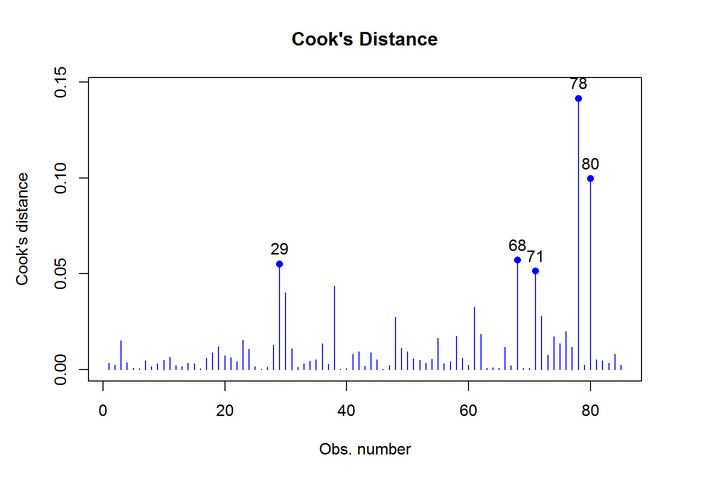
\includegraphics[width=0.7\linewidth]{images/CooksDistancePlot-JS-Roy}
	\caption{}
	\label{fig:CooksDistancePlot-JS-Roy}
\end{figure}

\begin{figure}[h!]
	\centering
	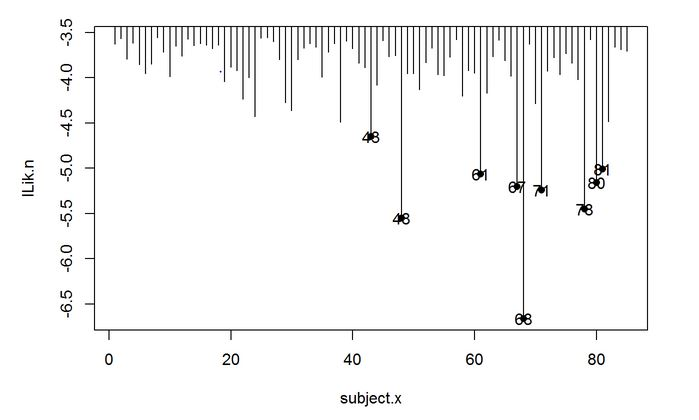
\includegraphics[width=0.7\linewidth]{images/LogLik-JS-Roy}
	\caption{}
	\label{fig:LogLik-JS-Roy}
\end{figure}

As the model is structurally different from the models discussed in the earlier sections, Residual analysis will be briefly revisited.
\begin{figure}[h!]
	\centering
	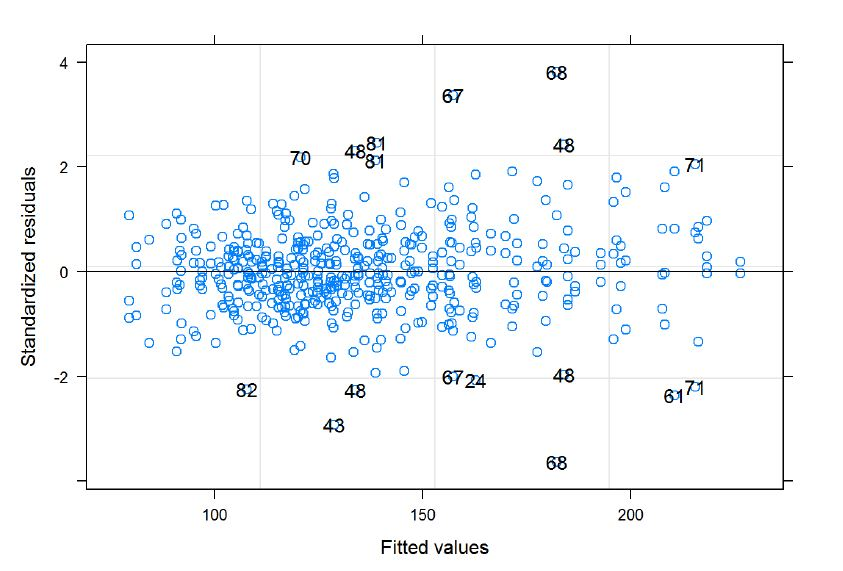
\includegraphics[width=0.7\linewidth]{images/Residuals-JS-Roy}
	\caption{}
	\label{fig:Residuals-JS-Roy}
\end{figure}

\newpage
\section{Case Deletion Diagnostics for the Variance Ratios}
%- H Case Deletion Diagnostics 

Schabenberger advises on the use of deletion diagnostics for variance components of an LME model.
Taking the core principals of his methods, and applying them to the Method Comparison problem, case deletion diagnostics are used on the variance components of the Roy model., specifically the ratio of between subject variances and the within subject covariances respecitvely.


\[ \mbox{BSVR} = \frac{\sigma^2_2}{\sigma^2_2} \phantom{makespace}  \mbox{WSVR} = \frac{d^2_2}{d^2_2} \]

These variance ratios are re-computed for each case removed, and may be analysed seperately or jointly for outliers. 

The Grubbs' Test for Outliers is a commonly used technique for assessing outlier in a univariate data set. As there may be several outliers (i.e. influential cases) present, the Grubbs test is not useful. However, as identification is all that is required, a simple outlier detection technique, such as using to Tukey's specification for boxplots (i.e. greater than $Q_3 +1.5 IQR$ or less than $Q_1 - 1.5 IQR$), will suffice. Ranking the asbolute values of the standardizaed scores can also can be used to identify influential cases, even if the data is not normally distributed.

Bivariate Analyses may be applied jointly to the both sets of data sets, e.g. Mahalanobis distances. The Mahalanobis distance, while not an intuitive measure in the context of the data, can be used to rank highly influential cases. 

%============================================================================= %

\section*{Leave-One-Out Diagnostics with \texttt{lmeU}}
Galecki et al discuss the matter of LME influence diagnostics in their book, although not into great detail.


The command \texttt{lmeU} fits a model with a particular subject removed. The identifier of the subject to be removed is passed as the only argument

A plot ofthe per-observation diagnostics individual subject log-likelihood contributions can be rendered.

\subsubsection*{Likelihood Displacement}
%% Page 503 Galecki

\subsection{Likelihood Distances}

The \index{likelihood distance} likelihood distance is a global summary measure that expresses the joint influence of the subsets of observations, $U$, on all parameters in $\phi$ that were subject to updating. For classical linear models, the implementation of influence analysis is straightforward. \citet{schab} points out the likelihood distance gives the amount by which the log-likelihood of the model fitted from the full data changes if one were
to estimate the model from a reduced-data estimates. Importantly $LD(\psi_{(U)})$ is not the log-likelihood obtained by fitting the model to the reduced data set. It is obtained by evaluating the likelihood function based on the full data set (containing all $n$ observations) at the reduced-data estimates.


%---------------------------------------------------------- %
%Likelihood Displacement.
\[  LD(\boldsymbol{(U)})= 2[l\boldsymbol{\hat{(\phi)}} - l\boldsymbol{\hat{\phi}_\omega} ] \]
\[  RLD(\boldsymbol{(U)})= 2[ l_R\boldsymbol{\hat{(\phi)}} - l_R\boldsymbol{\hat{(\phi)}_\omega} ] \]
%	Large values indicate that $\boldsymbol{\hat{\theta}}$ and $\boldsymbol{\hat{\theta}_\omega}$ differ considerably.


An overall influence statistic measures the change in the objective function being minimized. For example, in
OLS regression, the residual sums of squares serves that purpose. In linear mixed models fit by
\index{maximum likelihood} maximum likelihood (ML) or \index{restricted maximum likelihood} restricted maximum likelihood (REML), an overall influence measure is the \index{likelihood distance} likelihood distance \citep{cook}. In LME models, fitted by either ML or REML, an important overall
influence measure is the likelihood distance \citep{cook82}. The  procedure requires the calculation of the full data estimates
$\hat{\psi}$ and estimates based on the reduced data set  $\hat{\psi}_{(U)}$. The likelihood distance is given by
determining


\begin{eqnarray}
LD_{(U)} &=& 2\{l(\hat{\psi}) - l( \hat{\psi}_{(U)}) \}\\
RLD_{(U)} &=& 2\{l_{R}(\hat{\psi}) - l_{R}(\hat{\psi}_{(U)})\}
\end{eqnarray}
%----schabenberger page 8
For classical linear models, the implementation of influence analysis is straightforward.
However, for LME models, the problem is more complex. Update formulas for the fixed effects are available only when the covariance parameters are assumed to be known. A measure of total influence requires updates of all model parameters. This can only be achieved in general is by omitting observations or cases, then refitting the model. This is a very simplistic approach, and computationally expensive.

\citet{west} examines a group of methods that examine various aspects of influence diagnostics for LME models.
For overall influence, the most common approaches are the \textit{likelihood distance} and the \textit{restricted likelihood distance}.

\subsubsection{The \texttt{logLik} Function}
\texttt{logLik.lme} returns the log-likelihood value of the linear mixed-effects model represented by object evaluated at the estimated coefficients. It is also possible to determine the restricted log-likelihood, if relevant, using this function. For the Blood Data Example,  the loglikelihood of the JS.roy1 model can be computed as follows.
\begin{framed}
	\begin{verbatim}
	> logLik(JS.roy1)
	'log Lik.' -2030.736 (df=8)
	\end{verbatim}
\end{framed}
%======================================================================================= %
	
\section{Likelihood Distance} %1.11
The \index{likelihood distance} likelihood distance is a global, summary measure, expressing the joint influence of the observations in the set $U$ on all parameters in $\phi$  that were subject to updating.

The likelihood distance gives the amount by which the log-likelihood of the full data changes if one were
to evaluate it at the reduced-data estimates. The important point is that $l(\psi_{(U)})$ is not the log-likelihood
obtained by fitting the model to the reduced data set.

It is obtained by evaluating the likelihood function based on the full data set (containing all n observations) at the reduced-data estimates.

The likelihood distance is a global, summary measure, expressing the joint influence of the observations in
the set $U$ on all parameters in $\psi$  that were subject to updating.
%------------%







%------------------------------%
%%%%%%%%%%%%%%%%%%%%%%%%%%%%%%%%%%%%%%%%%%%%%%%%%%%%%%%%%%%%%%%%%%%%%%%%%%%%%%%%%%%%%%%%%%%%%%%% Complex Data

%
%\section{Likelihood Distance} %1.11
%The \index{likelihood distance} likelihood distance is a global summary measure that expresses the joint influence of the subsets of observations, $U$, on all parameters in $\phi$ that were subject to updating. \citet{schab} points out the likelihood distance gives the amount by which the log-likelihood of the model fitted from the full data changes if one were
%to estimate the model from a reduced-data estimates. Importantly $LD(\psi_{(U)})$ is not the log-likelihood obtained by fitting the model to the reduced data set. It is obtained by evaluating the likelihood function based on the full data set (containing all $n$ observations) at the reduced-data estimates.
%
%
%%---------------------------------------------------------- %
%%Likelihood Displacement.
%\[  LD(\boldsymbol{(U)})= 2[l\boldsymbol{\hat{(\phi)}} - l\boldsymbol{\hat{\phi}_\omega} ] \]
%\[  RLD(\boldsymbol{(U)})= 2[ l_R\boldsymbol{\hat{(\phi)}} - l_R\boldsymbol{\hat{(\phi)}_\omega} ] \]
%%	Large values indicate that $\boldsymbol{\hat{\theta}}$ and $\boldsymbol{\hat{\theta}_\omega}$ differ considerably.




%---------------------------------------------------------------------------%



\chapter{Cook's Distance}

		\section{Cook's Distance for LMEs} %1.10

		
Diagnostic methods for fixed effects are generally analogues of methods used in classical linear models.
Diagnostic methods for variance components are based on `one-step' methods. \citet{cook86} gives a completely general method for assessing the influence of local departures from assumptions in statistical models. \citet{cook77} greatly expanded the study of residuals and influence measures. Cook's key observation was the effects of deleting each observation in turn could be computed without undue additional computational expense. Consequently deletion diagnostics have become an integral part of assessing linear models.	


% %- OLS
\index{Cook's Distance} Cooks Distance ($D_{i}$) is a well known diagnostic technique used in classical linear models, that functions an overall measure of the combined impact of the $i$th case of all estimated regression coefficients. It uses the same structure for measuring the combined impact of the differences in the estimated regression coefficients when the $i$th case is deleted. $D_{(i)}$ can be calculated without fitting a new regression coefficient each time an observation is deleted. Importantly, $D_{(i)}$ can be calculated without fitting a new regression coefficient each time an observation is deleted.
		
\index{Cook's distance} Cook's $D$ statistics (i.e. colloquially Cook's Distance) is a measure of the influence of observations in subset $U$ on a vector of parameter estimates \citep{cook77}.
		
\[ \delta_{(U)} = \hat{\beta} - \hat{\beta}_{(U)}\]
		
If V is known, Cook's D can be calibrated according to a chi-square distribution with degrees of freedom equal to the rank of $\boldsymbol{X}$ \citep{cpj92}. (\textbf{State V and X})
		
		
% %- Interpretation
Cook's distance can be used in several ways: to indicate data points that are particularly worth checking for validity; to indicate regions of the design space where it would be good to be able to obtain more data points. 
Large values for Cook's distance indicate observations for special attention. 

Use of threshold value for Cook's Distance is discouraged (\textbf{cite: JohnFox}). However, informal heuristics do exist for OLS models; Obervations for which Cook's distance is higher than 1 are to be considered as influential. Alternatively there is an informal threshold of $4/N$ or $4/(N−k−1)$, where N is the number of observations and k the number of explanatory variables.

% Interpretation
% http://stats.stackexchange.com/questions/22161/how-to-read-cooks-distance-plots %

% Fox, John. (1991). Regression Diagnostics: An Introduction. Sage Publications.

\textbf{cite: JohnFox} advises the use of diagnostic plotting and to examine in closer details the points with "\textit{values of D that are substantially larger than the rest}", and that thresholds should just be used to enhance graphical displays.


The effect on the precision of estimates is separate from the effect on the point estimates. Data points that have a small \index{Cook's distance}Cook's distance, for example, can still greatly affect hypothesis tests and confidence intervals, if their  influence on the precision of the estimates is large.

%
%\subsubsection{Interpretation}
%Specifically $D_i$ can be interpreted as the distance one's estimates move within the confidence ellipsoid that represents a region of plausible values for the parameters.[clarification needed] This is shown by an alternative but equivalent representation of Cook's distance in terms of changes to the estimates of the regression parameters between the cases where the particular observation is either included or excluded from the regression analysis.
%
%================================================ %
% %- Exention to LMEs
\citet{CPJ} would later adapt the \index{Cook's distance}Cook's Distance measure for the analysis of LME models. For LME models, two formulations exist; a \index{Cook's distance}Cook's distance that examines the change in fixed fixed parameter estimates, and another that examines the change in random effects parameter estimates. The outcome of either Cook's distance is a scaled change in either $\beta$ or $\theta$.

For LME models, Cook's distance can be extended to model influence diagnostics by defining.
 
 \[ CD_{\beta i} = {(\hat{\beta} - \hat{\beta}_{[i]})^{T}(\boldsymbol{X}^{\prime}\boldsymbol{V}^{-1}\boldsymbol{X}) (\hat{\beta} - \hat{\beta}_{[i]}) \over p}\]
 
 It is also desirable to measure the influence of the case deletions on the covariance matrix of $\hat{\beta}$.
 
		
\citet{schabenberger} discusses a taxonomy of Cook's distance when applied to LME models. \begin{itemize}
	\item For variance components $\gamma$: $CD(\gamma)_i$,
	\item For fixed effect parameters $\beta$: $CD(\beta)_i$,
	\item For random effect parameters $\boldsymbol{u}$: $CD(u)_i$,
	\item For linear functions of $\hat{beta}$: $CD(\psi)_i$
\end{itemize}			
%============================================================================= %


It is also desirable to measure the influence of the case deletions on the covariance matrix of $\hat{\beta}$.
% % - Fixed Effects Parameter		

	For fixed effects parameter estimates in LME models, the \index{Cook's distance} Cook's distance can be extended to measure influence on these fixed effects.
	
	\[
	\mbox{CD}_{i}(\beta) = \frac{(c_{ii} - r_{ii}) \times t^2_{i}}{r_{ii} \times p}
	\]
	

For fixed effects parameter estimates in LME models, the \index{Cook's distance} Cook's distance can be extended to measure influence on these fixed effects.

\[
\mbox{CD}_{i}(\beta) = \frac{(c_{ii} - r_{ii}) \times t^2_{i}}{r_{ii} \times p}
\]
		
	For random effect estimates, the \index{Cook's distance} Cook's distance is
	
	\[
	\mbox{CD}_{i}(b) = g{\prime}_{(i)} (I_{r} + \mbox{var}(\hat{b})D)^{-2}\mbox{var}(\hat{b})g_{(i)}.
	\]
Large values for Cook's distance indicate observations for special attention.

A large value for $CD(u)_i$ indicates that the $i-$th observation is influential in predicting random effects.
For linear functions, $CD(\psi)_i$ does not have to be calculated unless $CD(\beta)_i$ is large.
%===================================================== %
		
		
		\subsection{Cook's Distance}
		\begin{itemize}
			\item For variance components $\gamma$: $CD(\gamma)_i$,
			\item For fixed effect parameters $\beta$: $CD(\beta)_i$,
			\item For random effect parameters $\boldsymbol{u}$: $CD(u)_i$,
			\item For linear functions of $\hat{beta}$: $CD(\psi)_i$
		\end{itemize}
		Diagnostic tool for variance components
		\[ C_{\theta i} =(\hat(\theta)_{[i]} - \hat(\theta))^{T}\mbox{cov}( \hat(\theta))^{-1}(\hat(\theta)_{[i]} - \hat(\theta))\]
		
		\begin{description}
			\item[Random Effects]	
			A large value for $CD(u)_i$ indicates that the $i-$th observation is influential in predicting random effects.
			\item[linear functions]
			$CD(\psi)_i$ does not have to be calculated unless $CD(\beta)_i$ is large.
		\end{description}
		


		
\subsubsection{Random Effects}

A large value for $CD(u)_i$ indicates that the $i-$th observation is influential in predicting random effects.

	
\subsubsection{linear functions}

$CD(\psi)_i$ does not have to be calculated unless $CD(\beta)_i$ is large.


%	\subsection{Information Ratio}
%	
%	\newpage
%	\section*{Cook's Distance} %1.9
%	
%Cook (1977)
\textit{Cook (1977)} greatly expanded the study of residuals and influence measures. Cook's key observation was the effects of deleting each observation in turn could be computed without undue additional computational expense. Consequently deletion diagnostics have become an integral part of assessing linear models.


Cook (1986) gave a completely general method for assessing influence of local departures from
assumptions in statistical models.



		
		
		
		
		%---------------------------------------------------------------------------%
		\section{Cook's Distance for LMEs} %1.10
	
	
		
%============================================================================= %

\subsection{Cook's Distance}%1.9.3

For linear mixed effects models, Cook's distance can be extended to model influence diagnostics by definining.

\[ C_{\beta i} = {(\hat{\beta} - \hat{\beta}_{[i]})^{T}(\boldsymbol{X}^{\prime}\boldsymbol{V}^{-1}\boldsymbol{X}) (\hat{\beta} - \hat{\beta}_{[i]}) \over p}\]

It is also desirable to measure the influence of the case deletions on the covariance matrix of $\hat{\beta}$.







\subsection{Cooks's Distance}%1.9.2
\index{Cook's distance} Cook's $D$ statistics (i.e. colloquially Cook's Distance) is a measure of the influence of observations in subset $U$ on a vector of parameter estimates \citep{cook77}.

\[ \delta_{(U)} = \hat{\beta} - \hat{\beta}_{(U)}\]

If V is known, Cook's D can be calibrated according to a chi-square distribution with degrees of freedom equal to the rank of $\boldsymbol{X}$ \citep{cpj92}.


For LME models, Cook's distance can be extended to model influence diagnostics by defining.

%\[ C_{\beta i} = {(\hat{\beta} - \hat{\beta}_{[i]})^{T}(\boldsymbol{X}^{\prime}\boldsymbol{V}^{-1}\boldsymbol{X}) (\hat{\beta} - \hat{\beta}_{[i]}) \over p}\]

It is also desirable to measure the influence of the case deletions on the covariance matrix of $\hat{\beta}$.

\newpage
\bibliographystyle{chicago}
\bibliography{DB-txfrbib}


\end{document}

%---------------------------------------------------------------------------------------------------%


